\documentclass[10pt, letter]{article}
\newcommand{\doctitle}{%
Solving Raven's Test of Intelligence using Visual Representation}
\newcommand{\bigO}{\ensuremath{\mathcal{O}}}
\newcommand{\tab}{\hspace*{12em}}
\usepackage{graphicx}
\usepackage{float}
\usepackage{listings}
\usepackage{comment}
\usepackage{fancyvrb}
\usepackage{booktabs}
\usepackage[usenames,dvipsnames]{color}
\usepackage[center]{caption}
\usepackage{algorithm}
\usepackage{algpseudocode}
\usepackage[margin=1in]{geometry}
\usepackage[usenames,dvipsnames]{color}
\usepackage{hyperref}
\hypersetup{
  colorlinks,
  citecolor=Violet,
  linkcolor=Black,
  urlcolor=Blue}
\begin{document}
\title{\textbf{\doctitle}\\
\textsc{Project \#3}
}
  \author {Arvind Krishnaa Jagannathan \\ GT ID: 902891874}
   \date{October 30, 2012}
\maketitle

\section{Introduction}
\subsection*{Raven's Test for Intelligence}
Raven's test for intelligence usually involves questions of the type A:B::C:x, where A,B,C are usually images which have some implicit relations. x is an unknown image, which needs to be selected from a set of given options, based on which of the choices best ``fit'' into the inferred relation. The goal of this project is to be able to correctly solve 6 (+2) such problems, by representing each image as a visual representation, and deriving the relation through this representation.
\subsection*{Representation of problems for the Raven's Test}
This project aims to solve the Raven's Test for Intelligence purely by using visual representations. For more efficient processing in addition to being a time saving technique, instead of using the entire problem image as the visual representation, the GIF file of a given problem is split up into several images, each representing one frame of the problem statement. The split up files are categorized into two: (a) Reference (b) Solution. The image files for each problem is placed by convention as depicted in Figure \ref{fig2}.

\begin{figure}[h!]
  \centering
    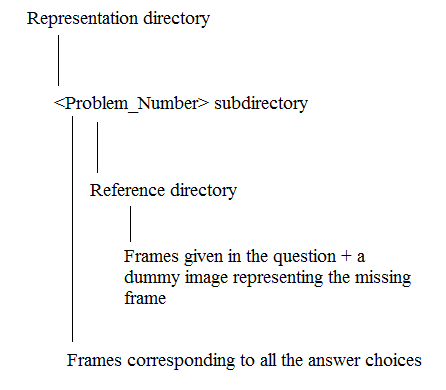
\includegraphics[scale = 0.6]{Images/Fig2}
    \caption{Structure of the visual representation directory}
  \label{fig2}
\end{figure}

The dummy image is placed in the Reference directory in order to procedurally infer the dimensions of the problem, which will be elaborated in the next section.

\begin{figure}[h!]
  \centering
    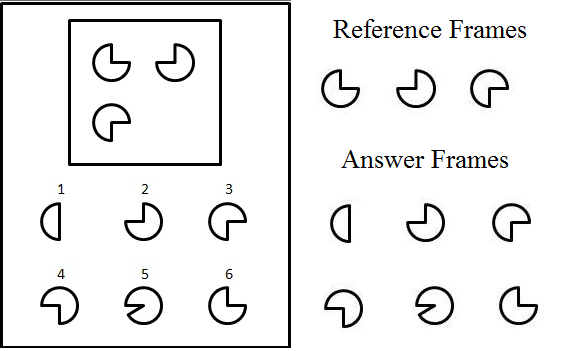
\includegraphics[scale = 0.5]{Images/Fig1}
    \caption{Visual Representation of a problem used in this project}
  \label{fig1}
\end{figure}

\section{Design of the Problem Solver}
\subsection*{Some Key Assumptions}
The program was designed to solve problems of visual reasoning in a way I would typically solve them. Although I was unable to capture every step in my reasoning process,  I have assumed that some particular parts of my reasoning approach would be universal and the program has incorporated that. 
	\subsubsection*{Assumption \#1}
Frames are usually inspected from left to right in a particular row. I assume that the first frame would act as a sort of ``base" frame and any differences or transitions of subsequent frames can be described with respect to the properties of this frame.
	\subsubsection*{Assumption \#2}
In problems of dimensions 3x3, I have assumed that if we find an answer such transitions in that row correspond to those in rows 1 and 2 of the reference matrix, then that is the answer. In other words, I have assumed that if row correspondence match, then column correspondence would ``fall-in-place''.
	\subsubsection*{Assumption \#3: Image correctness}
The visual analogy solver works on a pixel-by-pixel match in order to find the relevant structural transition from one frame to another. In most real world image formats, random pixels may appear out of place in the image due to the compression algorithm used (in my case JPG). For the best results, it is assumed that each of the visual representations for a given problem is ``noise free''. To achieve this, each image has been manually processed to remove as much of noise as possible.
	\subsubsection*{Assumption \#4: Image orientation and size}
This assumption is also a result of the visual analogy solver working on the level of pixels. Each of the individual frames are expected to be of exactly the same dimensions. In this project each frame has a dimension of 79x79 pixels. Although it is not necessary for the dimensions to be that of a square, it is vital that the number of pixels to compare are the same (hence the restriction on the dimensions). It is also assumed that the orientation of the frame is reproduced exactly as it is the problem, suited to fit the dimensions of the visual representation. This means that the amount of whitespace around the shapes, the alignment of each shape and the relative distance between the shapes of each frame from the original problem GIF image need to be preserved in the 79x79 representation. Figure \ref{fig3} represents the correct reproduction of the problem frame, as well as a few ``incorrect'' ones. The rectangular border around each orientation is just to give an idea of the position of the frame with respect to the dimensions of the representation; the actual representation does not contain this.
\begin{figure}[h!]
  \centering
    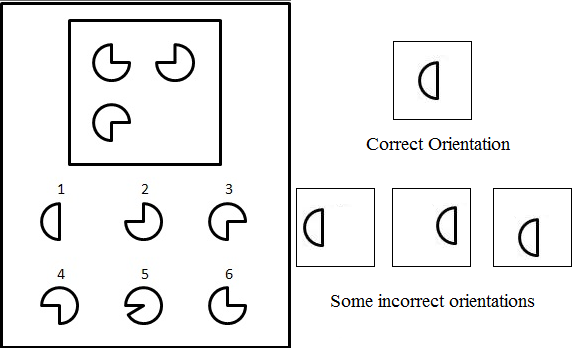
\includegraphics[scale = 0.5]{Images/Fig3}
    \caption{Preserving the relative characteristics of each frame}
  \label{fig3}
\end{figure}
	\subsubsection*{Assumption \#5: What is an exact match?}
Although two images seem to be matching exactly from a human point-of-view, when a pixel-by-pixel comparison is done, some finite difference may exist. Thus it is necessary to define certain thresholds within which if the pixel difference between two images fall, then they are considered to be matching. The following thresholds are established, experimentally, for various matching scenarios:
	\begin{enumerate}
		\item If image1 needs to checked for an exact match with image2 (i.e check if image1 == image2), then the comparison difference threshold is 200.
		\item If it needs to be checked if \\
		\centerline{Shapes(image1) - Shapes(image2) == Shapes(image3) - Shapes(image4)}\\
		then the threshold is 650.
		\item If it needs to be checked if \\
		\centerline{Shapes(image1) / Shapes(image2) == Shapes(image3) / Shapes(image4)}\\
		then the threshold is 50.
	\end{enumerate}
All these values are purely experimental (outlined in the \emph{Introspection} section) and may or may not be accurate since the number of problems used to arrive at these empirical values are very few.\\
\textbf{Note}: The pixel difference between two images is obtained as a correlation measure of the RGB matrix. It is mentioned in more detail in the subsequent section.
\subsubsection*{Assumption \#6}
In problems of visual reasoning people often find the ``macro'' differences between each frame, such as a missing shape or an addition of a new shape, before drilling down to ``micro'' differences such as the change in orientation, its color and so on. My program may not exhaustively capture all these differences, but it captures the ``macro'' differences and then uses that to filter the answer choices to a subset of the original choices, for which the ``micro'' differences are captured.
\subsection*{Algorithm}
The algorithm uses the idea that each frame in a given row or column of the problem matrix are connected by similitude transformations \cite{paper}. Thus the basic idea in this project is find the similitude transformation between the frames in each row of the reference matrix, apply that ``target'' transformation to the frame(s) in the ``incomplete'' row of the reference matrix and obtain the shape which is (most likely) the expected answer. Then each of the answer choices are compared with the expected shape to find the best match. In this project, the process of finding a similitude transformation is different for the case of 2x2 and 3x3 problems.

The steps of the algorithm are detailed below:

\subsubsection*{Step 0: Determining the dimensions of the problem}
The dimensions of the problem is determined by looking into the \textit{Reference} directory. Each frame in the reference matrix is stored as individual images. Hence if the dimension of the problem is NxN, since there is one frame missing in the reference matrix, the number of frames will be $N^2 - 1$. I am placing a dummy image \footnote{The dummy image is actually the GIF file provided for each of the problems} inside this directory so that in order to find the dimensionality of the problem, all the program needs to do is to count the number of elements in the \textit{Reference} directory and return its square root. Of course this project can only solve either 2x2 or 3x3 problems and reports an error if any other dimensionality is encountered.

Once the dimensionality of the problem is determined, two possible methods are defined depending on whether the problem is of 2x2 or 3x3 dimensions.

\subsection*{2x2 Problem}
For better explanation of the algorithm, let me define the convention for referring to the frames in the problem. The first frame of row 1 will be referred to as Frame1-1, the second as Frame 1-2. The first (and only) frame of row 2 will be referred to as Frame 2-1 and each of the answer choices will be referred as Frame1... Frame$N$ (Figure \ref{fig4}).

\begin{figure}[h!]
  \centering
    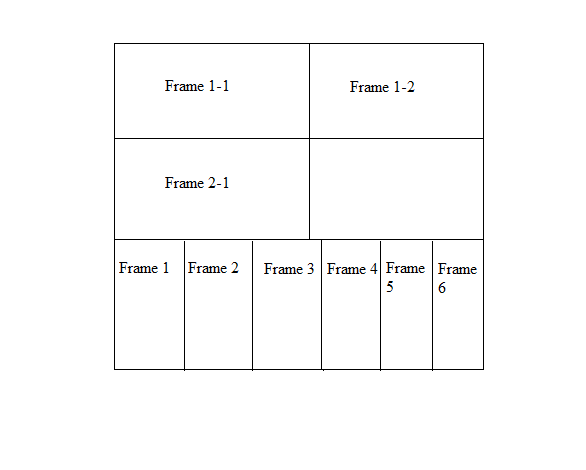
\includegraphics[scale = 0.5]{Images/Fig4}
    \caption{Convention for representing the frames in a 2x2 problem}
  \label{fig4}
\end{figure}

\subsubsection*{Step 1: Identifying the similitude transformations}
As per Kunda, McGreggor and Goel \cite{paper}, I have defined the following similitude transformations which can possibly exist between two given frames of the problem:
\begin{enumerate}
\item Identity
\item Reflection (w.r.t a vertical axis)
\item Flip (w.r.t a horizontal axis)
\item Rotation by $90\,^{\circ}$
\item Rotation by $180\,^{\circ}$
\item Rotation by $270\,^{\circ}$
\item Ratio between the number of shapes (on a pixel level!)
\item Addition/ removal of shapes (difference in the number of shapes) (again on the level of pixels)
\end{enumerate}

For clarity of understanding, I label transforms 1-6 as ``traditional'' transforms and 7-8 as ``non-traditional''. The process of finding the ``target'' transform is thus modified to find if it is ``traditional'' transform or ``non-traditional''. Depending on the category of transform, there will be a small change in the answer finding step.

To perform the visual comparison, each image corresponding to a frame is read from file and is stored as its associated RGB matrix. This is a square matrix (79x79) where the value of each element is equal to the RGB value of the corresponding pixel in the image. That is,\\
	\centerline{RGB Matrix A = $[a_{i,j}]$, where}\\
	\centerline{$[a_{i,j}]$ = RGBValue of $Pixel_{i,j}$ }\\
Since the image is black-and-white, the value of each element is either 0(black) or 255(white).

The RGB matrix of each of the frames are obtained and are used in determining the transformation being performed. To identify the particular transformation in play, each of the previously mentioned 8 transformations are checked (in that order) as follows:
\begin{enumerate}
\item \textbf{Identity}: 
\begin{enumerate}
\item Obtain the RGB matrices of frames 1-1(as F11) and 1-2(as F12). 
\item As a baseline for comparison obtain the self-corelation value of the RGB matrix of frame1-2. In general cross-corelation between two matrices (m1 and m2) are found as follows\footnote{As outlined in the SciPy documentation \cite{web}}
	\begin{itemize}
		\item Find the inner product of m1 with the convex combination matrix \cite{math} [299, 587, 114] to obtain the luminance value for each pixel.
		\item We perform the above step so that when divided by a constant (in my case 1000.0), the elements in the resulting matrix are normalized and lie in the range [0,1].
		\item Repeat the above steps for m2 as well. Now we have two resultant matrices, say M1 and M2.
		\item Apply the \emph{SciPy} function \cite{web} \emph{correlate2d}, with the parameters being M1 and M2, to obtain an array of floating point numbers, which represent various measures of corelation between the two matrices.
		\item The maximum value among the array is the corelation measure of M1 with M2 (and in turn m1 with m2).
	\end{itemize}
So to obtain the self-corelation of F12, replace both m1 and m2 in the procedure listed above with F12. Call this value as $selfCorelation$.
\item Obtain the cross-corelation value of F11 with F12, by replacing m1 with F11 and m2 with F12. Let this value be $crossCorelation\_Identity$.
\item Check for an exact match between $selfCorelation$ and $crossCorelation\_Identity$ (using the threshold described in Point 1 of Assumption 5)
\item If the difference is within permissible limits, report that the target transformation is `IDENTITY'.
\end{enumerate}
\textbf{Note}: For each of the ``traditional'' transformations, the first two steps described for \textsc{Identity} hold true. For the next transformations, I will be outlining the subsequent steps after finding the value of $selfCorelation$.
\item \textbf{Reflection}:
\begin{enumerate}
	\item Perform the reflection of frame1-1, using the \emph{PIL} utility \emph{transpose} \cite{pil} as,\\
		\hspace*{3cm}F11.transpose(FLIP\_LEFT\_RIGHT)
	\item Obtain the RGB matrix of this reflection and store it as F11$_{Reflection}$.
	\item Obtain the cross-corelation value of F11$_{Reflection}$ with F12. Let this value be $crossCorelation\_Reflection$.
	\item Check for an exact match between $selfCorelation$ and $crossCorelation\_Reflection$ (using the threshold described in Point 1 of Assumption 5)
	\item If the difference is within permissible limits, report that the target transformation is `REFLECTION'.
\end{enumerate}

\item \textbf{Flip}:
\begin{enumerate}
	\item Perform the vertical flipping of frame1-1, using the \emph{PIL} utility \emph{transpose} \cite{pil} as,\\
		\hspace*{3cm}F11.transpose(FLIP\_TOP\_BOTTOM)
	\item Obtain the RGB matrix of this flip and store it as F11$_{Flip}$.
	\item Obtain the cross-corelation value of F11$_{Flip}$ with F12. Let this value be $crossCorelation\_Flip$.
	\item Check for an exact match between $selfCorelation$ and $crossCorelation\_Flip$ (using the threshold described in Point 1 of Assumption 5)
	\item If the difference is within permissible limits, report that the target transformation is `FLIP'.
\end{enumerate}

\item \textbf{Rotation by $90\,^{\circ}$}:
\begin{enumerate}
	\item Perform the rotation of frame1-1 by $90\,^{\circ}$, using the \emph{PIL} utility \emph{rotate} \cite{pil} as,\\
		\hspace*{3cm}F11.rotate(90)
	\item Obtain the RGB matrix of this rotation and store it as F11$_{Rot90}$.
	\item Obtain the cross-corelation value of F11$_{Rot90}$ with F12. Let this value be $crossCorelation\_Rot90$.
	\item Check for an exact match between $selfCorelation$ and $crossCorelation\_Rot90$ (using the threshold described in Point 1 of Assumption 5)

	\item If the difference is within permissible limits, report that the target transformation is `ROTATE90'.
\end{enumerate}

\item \textbf{Rotation by $180\,^{\circ}$}:
\begin{enumerate}
	\item Perform the rotation of frame1-1 by $180\,^{\circ}$, using the \emph{PIL} utility \emph{rotate} \cite{pil} as,\\
		\hspace*{3cm}F11.rotate(180)
	\item Obtain the RGB matrix of this rotation and store it as F11$_{Rot180}$.
	\item Obtain the cross-corelation value of F11$_{Rot180}$ with F12. Let this value be $crossCorelation\_Rot180$.
	\item Check for an exact match between $selfCorelation$ and $crossCorelation\_Rot180$ (using the threshold described in Point 1 of Assumption 5)
	\item If the difference is within permissible limits, report that the target transformation is `ROTATE180'.
\end{enumerate}

\item \textbf{Rotation by $270\,^{\circ}$}:
\begin{enumerate}
	\item Perform the rotation of frame1-1 by $270\,^{\circ}$, using the \emph{PIL} utility \emph{rotate} \cite{pil} as,\\
		\hspace*{3cm}F11.rotate(270)
	\item Obtain the RGB matrix of this rotation and store it as F11$_{Rot270}$.
	\item Obtain the cross-corelation value of F11$_{Rot270}$ with F12. Let this value be $crossCorelation\_Rot270$.
	\item Check for an exact match between $selfCorelation$ and $crossCorelation\_Rot270$ (using the threshold described in Point 1 of Assumption 5)	
	\item If the difference is within permissible limits, report that the target transformation is `ROTATE270'.
\end{enumerate}

\textbf{Note}: If none of the ``traditional'' transforms have been reported, then it is necessary to find a good-enough match using \textbf{BOTH} the ``non-traditional'' transforms, one after another. In the case of a non-traditional transform, a particular metric (ratio between the number of shapes in frame1-1 and frame1-2 or the difference in the number of shapes between them) is obtained from the reference frame and it is matched against every possible ordered pair of 
		\\\hspace*{3cm}(frame2-1, frame$_i$), \\
where i is from 1 to $NumberOfAnswerChoices$. In such a case the answer choice ($i$) which gives the closest match (subject to the thresholds defined in Points 2 and 3 of Assumption 5 depending on the metric in question) is declared the right choice.

\item \textbf{Ratio between the number of shapes}:
\begin{enumerate}
	\item To obtain the ratio between frame1-1 and frame1-2, perform the following NumPy array operation,\\
		\hspace*{3cm} ratio = sum(sum(F11 / F12))
	\item Mark the ``target'' transform as `NON-TRADITIONAL'.
\end{enumerate}

\item \textbf{Addition/ Removal of shapes (Difference in number of shapes)}:
\begin{enumerate}
	\item To obtain the difference between frame1-1 and frame1-2, perform the following NumPy array operation,\\
		\hspace*{3cm} difference = sum(sum(F11 - F12))
	\item Mark the ``target'' transform as `NON-TRADITIONAL'.
\end{enumerate}
\end{enumerate}

\subsubsection*{Step 2: Identifying the answer choice}
Identify the nature of the ``target'' transform. If its type is NOT `NON-TRADITIONAL', then it is possible to generate the (most likely) expected answer by applying this target transform on frame2-1. The expected answer is checked against each of the answer choices until a best match is found. The following steps describe this procedure in more detail:
\begin{enumerate}
	\item Assign a matrix F$_{expected}$ which will hold the RGB matrix of the expected answer.
	\item Let F21 be the RGB matrix corresponding to the visual representation of frame2-1.
	\item If the target transform is IDENTITY, then \\
			\hspace*{3cm} F$_{expected}$ = F21.
	\item Else if the target transform is REFLECTION, then \\
			\hspace*{3cm} F$_{expected}$ = F21.transpose(FLIP\_LEFT\_RIGHT).
	\item Else if the target transform is FLIP, then \\
			\hspace*{3cm} F$_{expected}$ = F21.transpose(FLIP\_TOP\_BOTTOM).
	\item Else if the target transform is ROTATE90, then \\
			\hspace*{3cm} F$_{expected}$ = F21.rotate(90).
	\item Else if the target transform is ROTATE180, then \\
			\hspace*{3cm} F$_{expected}$ = F21.rotate(180).
	\item Else if the target transform is ROTATE270, then \\
			\hspace*{3cm} F$_{expected}$ = F21.rotate(270).
	\item Compute the self-corelation value of F$_{expected}$ (as outlined previously) and store it as $expected\_value$.
	\item For each of the answer choices, obtain the RGB matrix of the corresponding visual representation as F$_i$. For instance, the RGB matrix of choice 1 will be F$_1$.
	\item Obtain the cross-corelation of F$_i$ with F$_{expected}$. Store it as $actual\_value_i$.
	\item The answer choice $i$ for which the difference \\
				\hspace*{3cm} Abs($actual\_value_i$ - $expected\_value$) \\
			is the least is the correct answer.
\end{enumerate}

However, if the type of the transform is `NON-TRADITIONAL', then the following steps need to be carried out in order to find an answer choice.
\begin{enumerate}
	\item The ratio between the number of shapes in frame1-1 and frame1-2 is stored as $ratio$
	\item Perform the steps involved in computing $ratio$, replacing F11 with F21 and F12 with each of the answer choices F$_i$.
	\item Let $actual\_ratio_i$ correspond to the ratio of F21 with the answer choice F$_i$.
	\item As per Point 3 of Assumption 5, find those choices for which \\
				\hspace*{3cm} Abs($actual\_ratio_i$ - $ration$)\\	
	 fit within the threshold value of 50. If there is just one answer choice, then that is announced as the correct answer.
	\item If there is more than one choice which fits within the threshold, then for each choice $k$, find out the $actual\_difference_k$ similar to how $difference$ was computed.
		\begin{itemize}
			\item Among all $k$ find the one which for which the value of \\
				\hspace*{3cm} Abs($actual\_difference_k$ - $difference$) \\
			is the least. This choice is then announced as the correct answer.
		\end{itemize}
	\item If there is no choice which fits within the threshold, then for all possible answer choices $i$, find out $actual\_difference_i$ 
		\begin{itemize}
		\item Among all $i$ find the one which for which the value of \\
				\hspace*{3cm} Abs($actual\_difference_i$ - $difference$) \\
			is the least. If this is less than the threshold of 650 (Point 2 Assumption 5), then announce it as the answer. Otherwise, announce that none of the answers are right.
		\end{itemize}
\end{enumerate}

\subsection*{3x3 Problem}
The frame nomenclature for a 3x3 problem is an extension of that used for the 2x2 problem. It is illustrated in Figure \ref{fig5}. The answer choices will be labeled as Frame1...N.

\begin{figure}[h!]
  \centering
    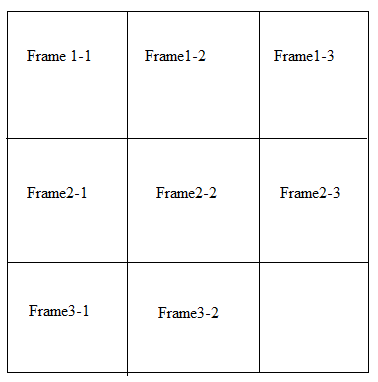
\includegraphics[scale = 0.5]{Images/Fig5}
    \caption{Convention for representing the frames in a 3x3 problem}
  \label{fig5}
\end{figure}

\subsubsection*{Step 1: Find the relation between frames of each row}
In case of a 3x3 problem, due to large permutation of the number of two frame combinations possible, I have not considered the ``traditional'' transformations. There are three ``non-traditional'' transformations which I have considered,
\begin{enumerate}
	\item Ratio between the number of shapes in frames 1-2 \& 1-3 and 2-2 \& 2-3.
	\item Difference between the number of shapes in frames 1-2 \& 1-3 and 2-2 \& 2-3.
	\item Difference in the number of shapes in 1-1, 1-2 \& 1-3.
\end{enumerate}
The third metric actually dominates the first two in obtaining the right answer, but it is also significantly more computationally intensive. Thus, I have used the first two metrics as ``macro'' filters, eliminating certain obviously incorrect choices. Thus instead of applying the third metric on all the answer choices, only those still remaining after the filtering stage need to be examined. The following sections describe how to obtain each of these metrics.

\subsubsection*{Obtaining the ratio of the number of shapes}
\begin{enumerate}
	\item Obtain the RGB matrix of the visual representations of frames 1-2 (as F12) and 1-3 (as F13). Similar to the 2x2 problem, compute the ratio between the number of shapes, using the \textit{NumPy} method \textit{sum} as \\
	\hspace*{3cm} ratio1 = sum(sum(F12 / F13))
	\item Similarly obtain the RGB matrix of the visual representations of frames 2-2 (as F22) and 2-3 (as F23). Compute the ratio between the number of shapes,\\
	\hspace*{3cm} ratio2 = sum(sum(F22 / F23))
	\item If the values of ratio1 and ratio2 match (within the threshold limit described in Point 3 of Assumption 5), then this metric will be used to filter out the answer choices. Otherwise it will not be used.
	\item If the metric is used, store the average of ratio1 and ratio2 in a variable $ratio$
\end{enumerate}

\subsubsection*{Obtaining the difference in the frames}
\begin{enumerate}
	\item Similar to the ratio, obtain the difference between F12 \& F13 and F22 \& F23 as follows, \\
	\hspace*{3cm} difference1 = sum(sum(F12 - F13))\\
	\hspace*{3cm} difference2 = sum(sum(F22 - F23))
	\item If the values of difference1 and difference2 match (within the threshold limit described in Point 2 of Assumption 5), then this metric will be used to filter out the answer choices. Otherwise it will not be used.
	\item If the metric is used, store the average of difference1 and difference2 in a variable $difference$
\end{enumerate}

\subsubsection*{Obtaining the pair-wise difference in the frames}
\begin{enumerate}
	\item Obtain the difference between F11 \& F12 and store it as difference12. \\
	\hspace*{3cm} difference12 = sum(sum(F11 - F12))
	\item Obtain the difference between F12 \& F13 and store it as difference23. \\
	\hspace*{3cm} difference23 = sum(sum(F12 - F13))
	\item Obtain the difference between F11 \& F13 and store it as difference13. \\
	\hspace*{3cm} difference13 = sum(sum(F11 - F13))	
\end{enumerate}

\subsubsection*{Step 2: Finding the correct answer choice}
For the given problem, all the above three metrics may be retained or just a subset of them. So the order of evaluating the answer choices and picking a correct one is as follows,
\begin{enumerate}
\item If the ratio metric can be used for the given problem, then
	\begin{enumerate}
		\item For all the answer frames F$_i$, compute the ratio with respect to frame3-2, i.e \\
		\hspace*{3cm} $actual\_ratio_i$ = sum(sum(F32 / F$_i$)) 
		\item Choose those answer choices for which \\
		\hspace*{3cm} Abs($actual\_ratio_i$ - $ratio$) $\langle$ 50\\
		and add it to the list of potential answers.
		\item If there is only one choice remaining, then declare that as the answer.
		\item If there are no choices, then all the choices are potential answers.
		\item Provided difference is a metric, perform a similar filtering on the potential answers using $difference$. That is, eliminate those choices for which \\
		\hspace*{3cm} Abs($actual\_difference_i$ - $difference$) $\rangle$ 650
		\item Again, if there is only once choice then declare it as the answer.
		\item If there are no choices, then all the choices still remain potential answers.
		\item Apply the pair-wise difference to each of the answer choices as follows, \\
		\hspace*{3cm} Compute diff12 = sum(sum(F31 - F32)) \\
		\hspace*{3cm} Compute diff23 = sum(sum(F32 - F$_i$)) \\
		\hspace*{3cm} Compute diff13 = sum(sum(F31 - F$_i$)) \\		
		\hspace*{3cm} $ReferenceSum$ = difference12 + difference23 + difference13 \\
		\hspace*{3cm} $AnswerSum$ = diff12 + diff23 + diff13 
		\item The choice for which the difference between $ReferenceSum$ and $AnswerSum$ is the least is declared as the right answer.
	\end{enumerate}
\item If the ratio metric cannot be used for the given problem and the difference metric can, then steps (e)-(i) from the previous technique can be applied to arrive at an answer.
\item If both the ratio and difference metric cannot be used, then perform only steps (h)-(i) to obtain the answer.
\end{enumerate}

\subsection*{Architecture of the Algorithm}
The overall visual solver's architecture is illustrated in Figure \ref{fig6} at a high level of abstraction. The 2x2 problem solver and the 3x3 problem solver are described in more detail in Figures \ref{fig7} and \ref{fig8}.

\begin{figure}[h!]
  \centering
    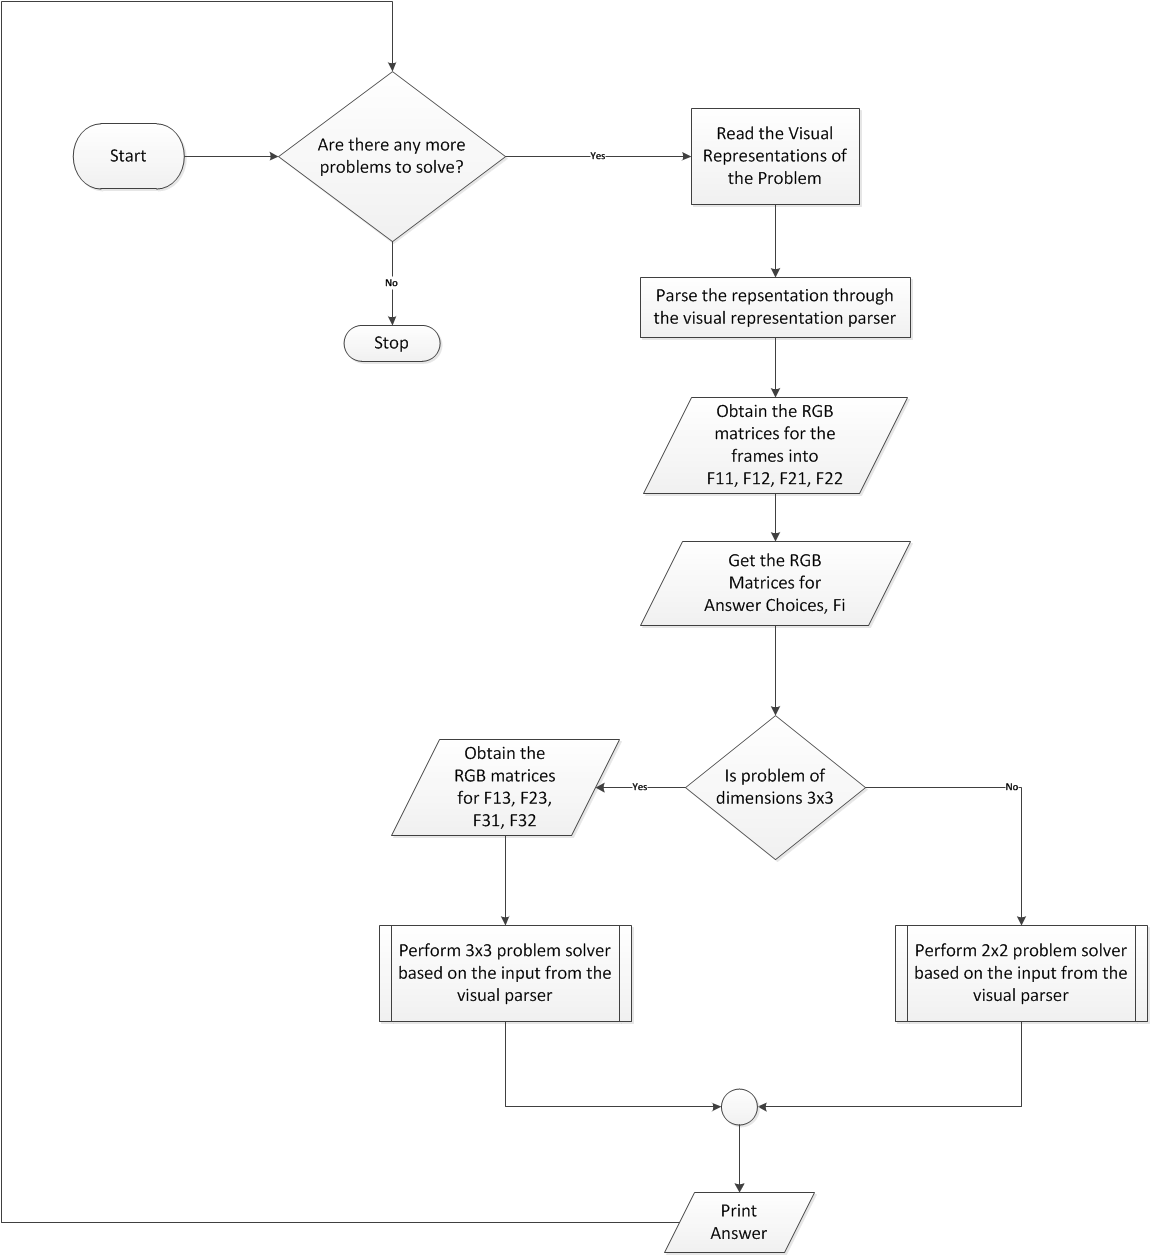
\includegraphics[scale = 0.35]{Images/Fig6}
    \caption{High-Level Architecture of the Visual Problem Solver}
  \label{fig6}
\end{figure}

\begin{figure}[h!]
  \centering
    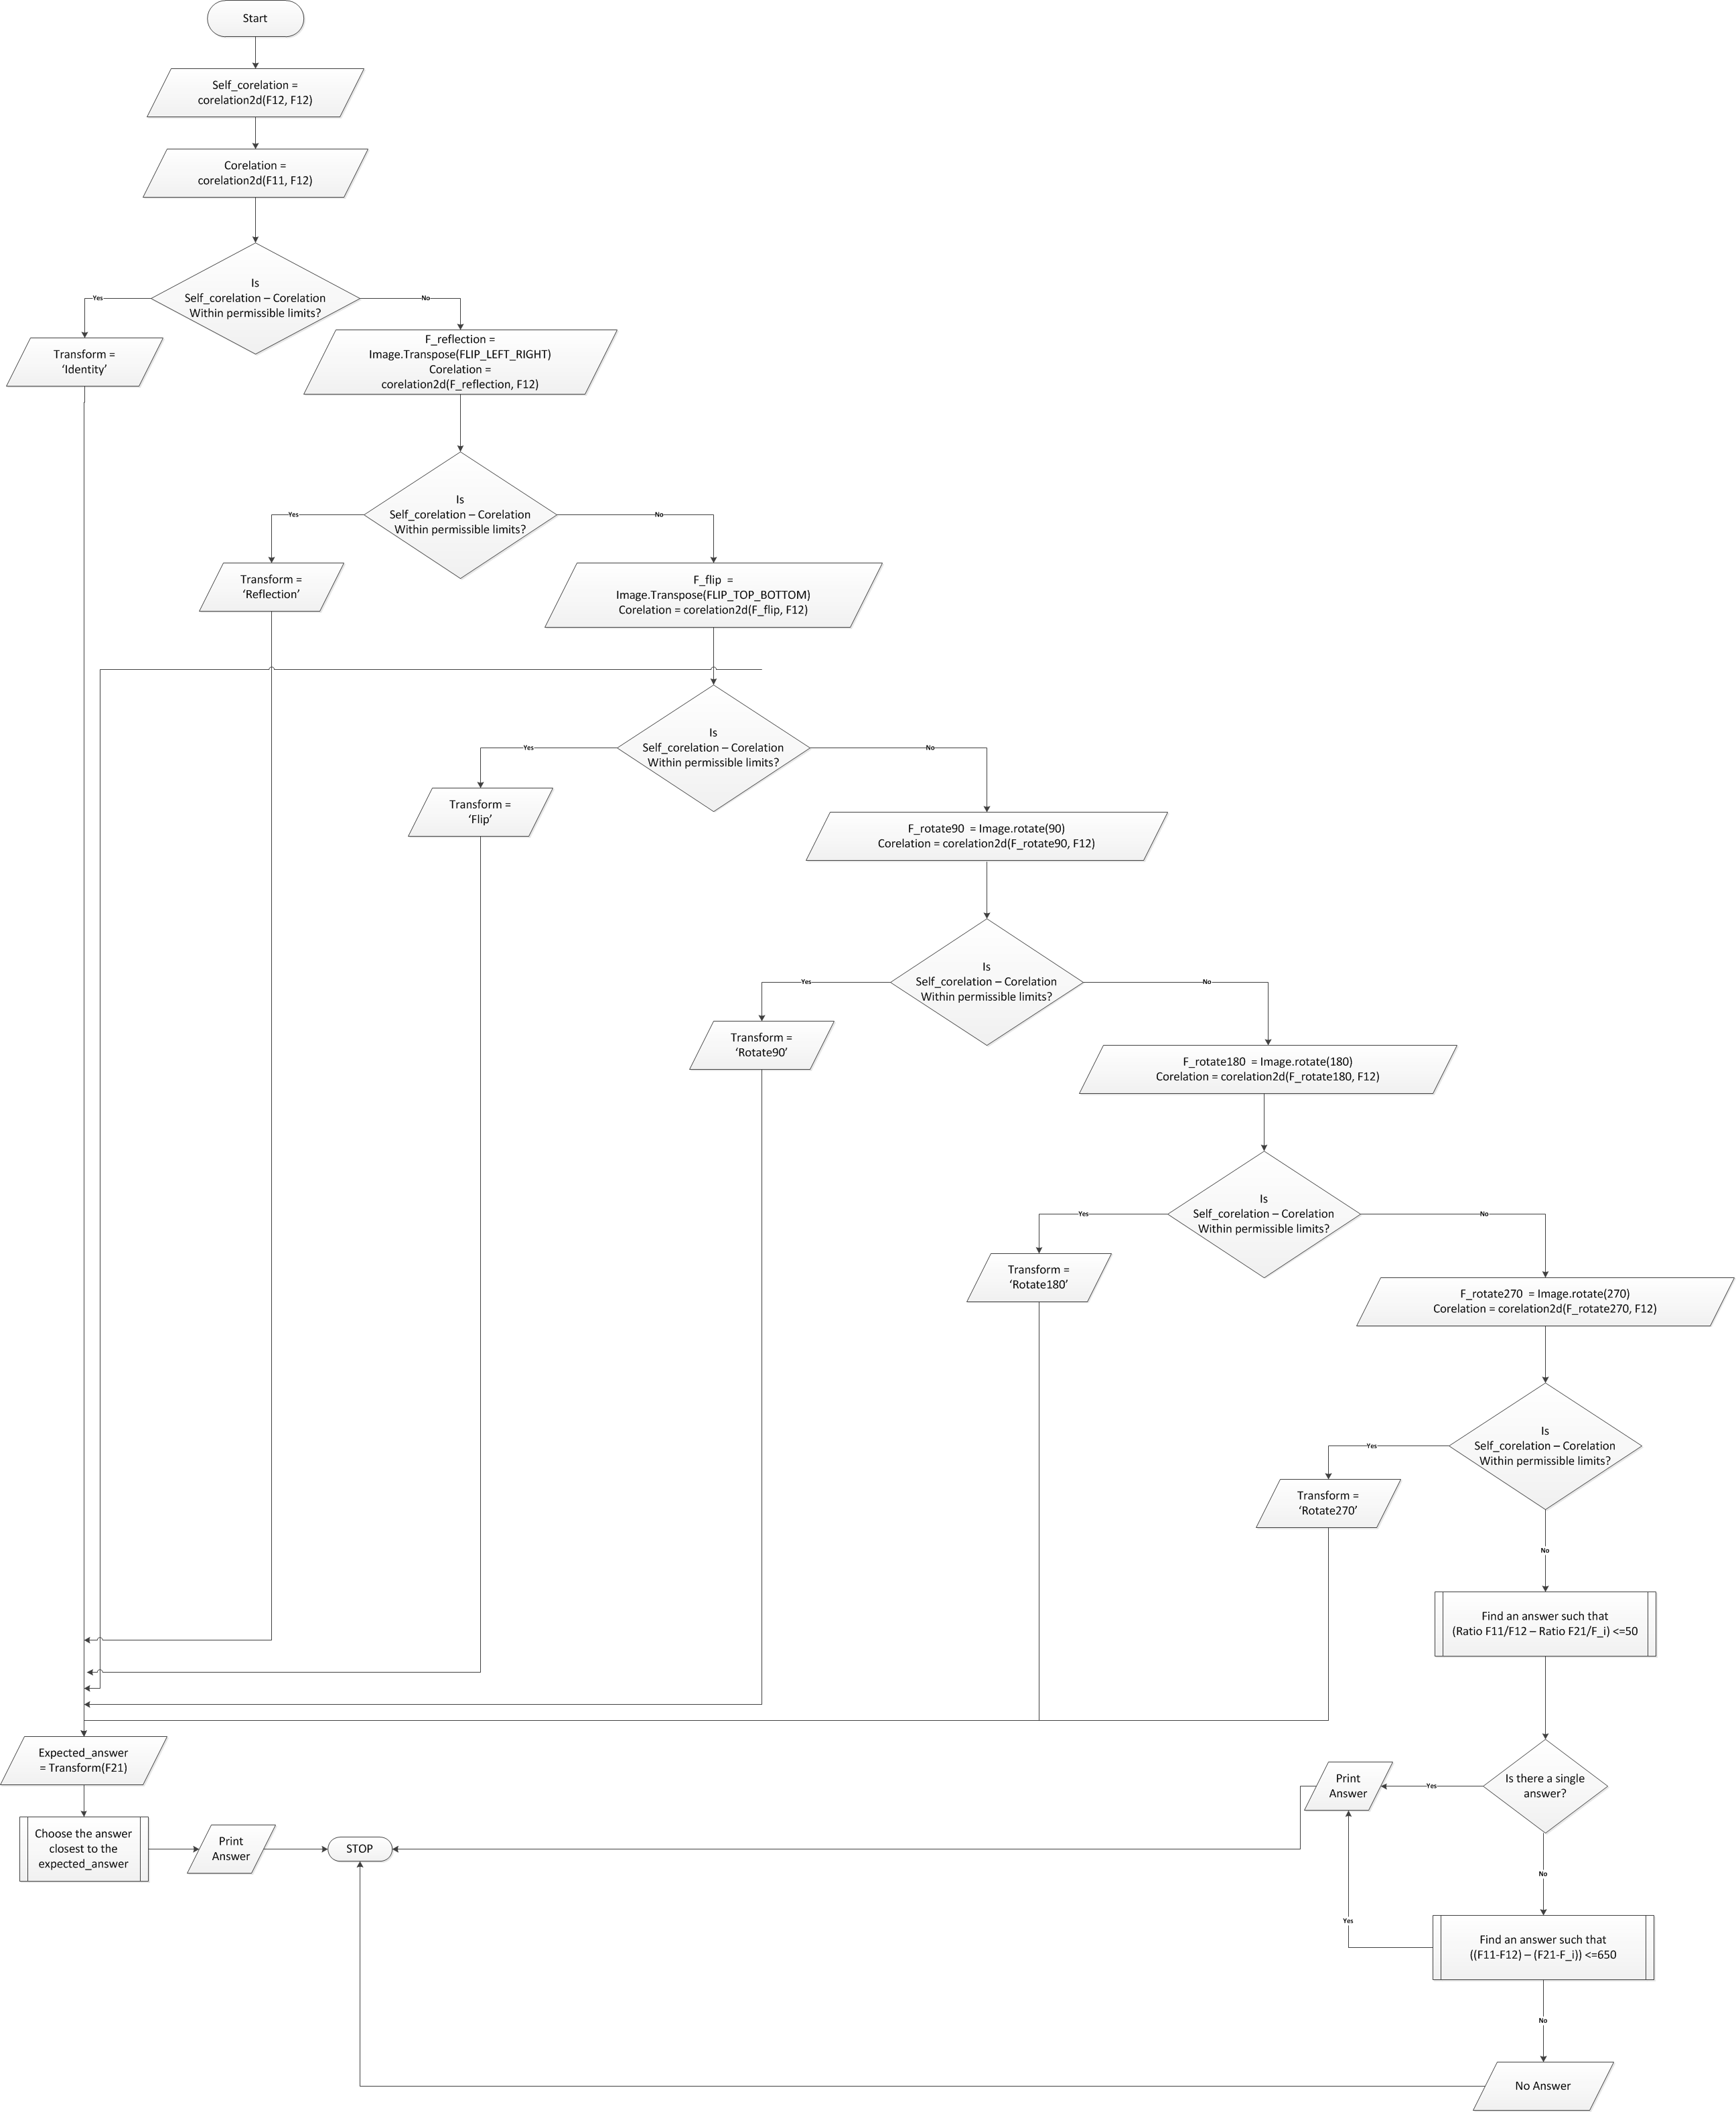
\includegraphics[scale = 0.25]{Images/Fig7}
    \caption{Architecture of the 2x2 Problem Solver}
  \label{fig7}
\end{figure}

\begin{figure}[h!]
  \centering
    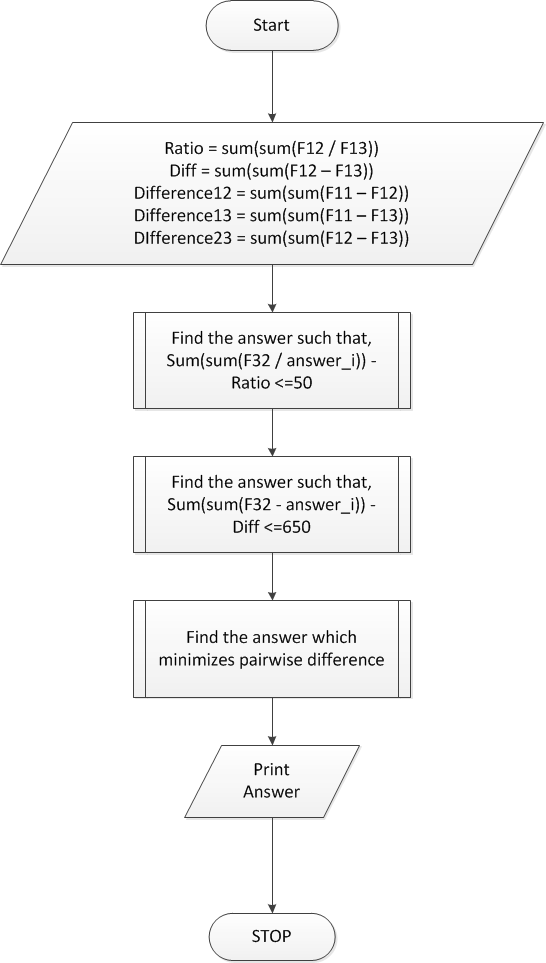
\includegraphics[scale = 0.35]{Images/Fig8}
    \caption{Architecture of the 3x3 Problem Solver}
  \label{fig8}
\end{figure}


\subsection*{Tracing the algorithm for a problem}
This section contains the trace of the algorithm for two instances of a 2x2 as well one instance of a 3x3 problem, each describing a salient aspect of the algorithm.
\subsubsection*{2x2 Problem - Example 1}
Figure \ref{fig9} represents a problem where one of the `traditional' transforms are used to determine the answer choice. The program proceeds as follows to find the answer,
\begin{figure}[h!]
  \centering
    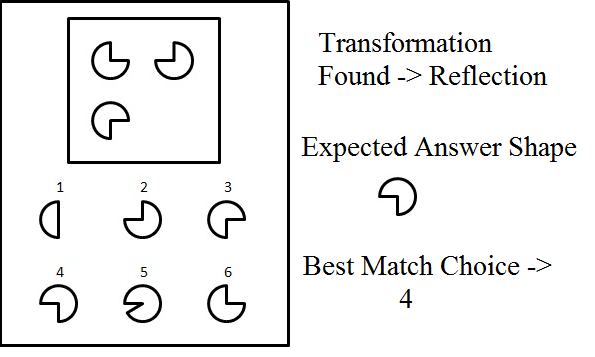
\includegraphics[scale = 0.5]{Images/Fig9}
    \caption{A sample 2x2 problem, with a `traditional' transformation}
  \label{fig9}
\end{figure}

\begin{enumerate}
	\item The 79x79 RGB matrix of frame1-1 and frame1-2 are stored as F11 and F12.
	\item The self-corelation value of F12 is found out to be 3844.0.
	\item For the identity transformation F11, the cross-corelation with F12 is found to be 1784.0.
	\item For the reflection transformation of F11, F\_Reflection, the cross-corelation with F12 is 3784.0. This is within the admissible threshold for equality and the transform is set to `REFLECT'.\\
	For the purpose of completeness the cross-corelation values for the other transforms are listed below,
	\begin{itemize}
		\item FLIP: 2881.0
		\item ROTATE90: 3691.0. \textbf{Note}: Although this transform also falls within the threshold, due to the fixed order in which the transforms are checked, reflection is given more priority over rotation.
		\item ROTATE180: 2901.0
		\item ROTATE270: 2004.0
	\end{itemize}
	\item Since the program has identified a `traditional' transformation, it does not bother with the non-traditional ones.
	\item Now the program formulates that the best expected answer should be a reflection of frame 2-1, which is also indicated in Figure \ref{fig9}.
	\item The self-corelation value for this image's RGB matrix (say F) is found to be 3884.0
	\item Each of the answer choices are represented by their RGB matrices and the cross-corelation with F is found out. They are listed out below,
		\begin{itemize}
			\item Choice 1: 2187.0
			\item Choice 2: 3458.0
			\item Choice 3: 4204.0
			\item Choice 4: 3803.0
			\item Choice 5: 4487.0
			\item Choice 6: 3689.0
		\end{itemize}
	\item Obviously the best match with the expected answer is choice 4, which turns out to be the right answer.
\end{enumerate}

\subsubsection*{2x2 Problem - Example 2}
In the example shown in Figure \ref{fig10}, none of the traditional transforms will give the right result. Again for the purpose of completeness, the significant comparison metrics for the 6 traditional transforms are given in the following list.

\begin{figure}[h!]
  \centering
    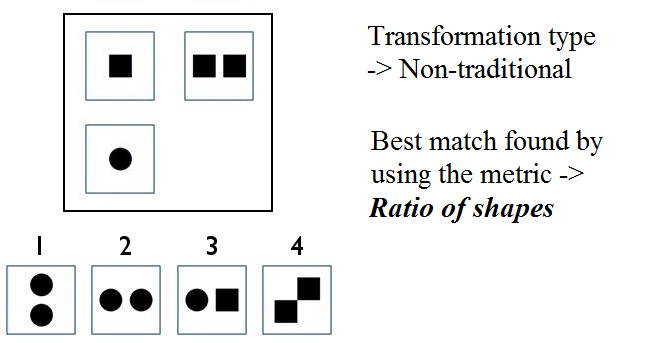
\includegraphics[scale = 0.5]{Images/Fig10}
    \caption{A sample 2x2 problem, with a `non-traditional' transformation}
  \label{fig10}
\end{figure}

\begin{enumerate}
	\item Self-corelation of frame1-2 : 1879.0
	\item Cross-corelation for IDENTITY : 2890.0
	\item REFLECTION : 2910.0
	\item ROTATE90 : 2453.0
	\item ROTATE180 : 2109.0
	\item ROTATE270 : 2907.0
\end{enumerate}

Obviously, none of the traditional transforms are even close to uncovering the true relation existing between frames1-1 and 1-2. Now the non-traditional transforms are applied.
\begin{itemize}
\item First the ratio between the shapes of frame1-1 and frame1-2 are found. The measure for this metric in this problem is found to be 729.0
\item The corresponding metric is computed for every pair involving frame2-1 and one of the answer choices. The values are as follows,
	\begin{enumerate}
		\item Ratio (Frame2-1, Choice 1): 604.0
		\item Ratio (Frame2-1, Choice 2): 731.0
		\item Ratio (Frame2-1, Choice 3): 575.0
		\item Ratio (Frame2-1, Choice 4): 834.0
	\end{enumerate}
\item From the listed values clearly choice 2 is the only choice within the threshold of 50. Hence it is declared as the result.\\
\textbf{Note}: Suppose the difference metric were applied to this problem instead of the ratio metric, the following values would have been obtained:
	\begin{enumerate}
		\item Diff(Frame1-1, Frame1-2): 1797.0
		\item Diff(Frame2-1, Choice 1): 907.0
		\item Diff(Frame2-1, Choice 2): 888.0
		\item Diff(Frame2-1, Choice 3): 1498.0
		\item Diff(Frame2-1, Choice 4): 1033.0
	\end{enumerate}
In such a scenario choice 3 would have been chosen as the right answer. It is just because I have given a higher priority to the ratio metric, choice 2 is chosen.\\
\textbf{Observation}: From the note it is clear that there can be two ways of viewing this problem. One is to say that with respect to the frame on the left, the number of shapes in the right frame has doubled (which is essentially what the ratio metric does). The second line of thought is to think that with respect to the left frame, a square has been added to the right frame (this is what the difference metric does). Hence depending on the line of thought, two possible solutions are possible, but it is purely out of personal taste that I have given more weight to the ratio metric than the difference metric (similar to the preference of reflection over rotation).
\end{itemize}
\subsubsection*{3x3 Problem - Example}
Compared to problems 4 and 6, problem 5, illustrated in Figure \ref{fig11} is tougher computationally. The trace of the algorithm through this problem will provide a sufficiently maximal example.

\begin{figure}[h!]
  \centering
    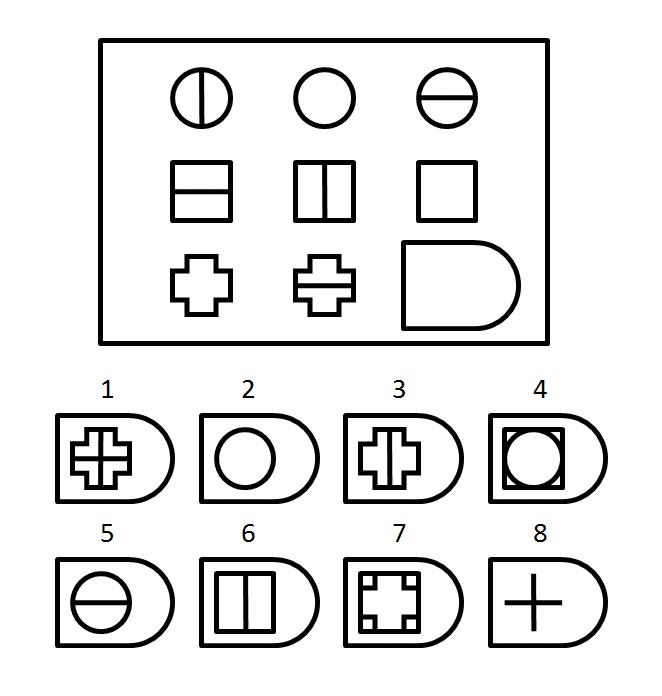
\includegraphics[scale = 0.25]{Images/Fig11}
    \caption{A computationally tough 3x3 problem}
  \label{fig11}
\end{figure}

\begin{enumerate}
\item The ratio metric is computed between frames1-2 \& 1-3 (451.0) and frames2-2 \& 2-3 (493.0). Since their difference is within the threshold, the ratio metric will be considered to filter out the answer choices.
\item The same is true of the difference metric too, since \\
	\hspace*{3cm}Diff frame1-2 - frame1-3 = 3451.0 and \\
	\hspace*{3cm}Diff frame2-2 - frame2-3 = 3309.0\\
	are within the threshold difference range (of 650.0).
\item The pairwise difference values are computed as follows, \\
	\hspace*{3cm}Diff frame1-1 - frame1-2 = 1931.0 and \\
	\hspace*{3cm}Diff frame1-2 - frame1-3 = 3451.0 and \\
	\hspace*{3cm}Diff frame1-1 - frame1-3 = 902.0
\item Applying the ratio metric for each pair of frame3-2 and the answer choices, we get the following values,
	\begin{enumerate}
		\item Ratio (frame3-2 / Choice 1): 509.0
		\item Ratio (frame3-2 / Choice 2): 149.0
		\item Ratio (frame3-2 / Choice 3): 464.0
		\item Ratio (frame3-2 / Choice 4): 613.0
		\item Ratio (frame3-2 / Choice 5): 198.0
		\item Ratio (frame3-2 / Choice 6): 704.0
		\item Ratio (frame3-2 / Choice 7): 402.0
		\item Ratio (frame3-2 / Choice 8): 453.0
		\end{enumerate}
\item From the above obtained values, choices 2, 4, 5, 6 are eliminated as they lie outside the defined threshold of 50 (from either 451.0 or 493.0)
\item Now for the remaining choices (1,3,7,8) the difference metric is applied, with the following results
	\begin{enumerate}
		\item Diff (frame3-2 - Choice 1): 4193.0
		\item Diff (frame3-2 - Choice 3): 3003.0
		\item Diff (frame3-2 - Choice 7): 4945.0
		\item Diff (frame3-2 - Choice 8): 3987.0		
	\end{enumerate}
\item In the above list, choices 1 and 7 fall outside the threshold range of 650.0 (from 3451.0 as well as 3309.0) and are subsequently eliminated.
\item The pairwise difference values are computed for the remaining choices (3 and 8) and the results are as follows
	\begin{enumerate}
		\item Diff (frame3-1 - frame3-2): 1731.0 (same for both answer choices obviously)
		\item Diff (frame 3-1 - Choice 3): 1210.0
		\item Diff (frame3-2 - Choice 3): 3003.0
		\item Diff (frame3-1 - Choice 8): 2890.0
		\item Diff (frame3-2 - Choice 8): 3987.0 
	\end{enumerate}
\item The $ReferenceSum$ = 1931.0 + 3451.0 + 902.0 = 6284.0
\item The $ChoiceSum$ for Choice 3 = 1731.0 + 1210.0 + 3003.0 = 5944.0
\item The $ChoiceSum$ for Choice 8 = 1731.0 + 2890.0 + 3987.0 = 8608.0
\item Obviously the difference between $ChoiceSum$ and $ReferenceSum$ is least for choice 3, which is declared as the right answer.
\end{enumerate}

\section{Implementation and Execution Details}

The entire project is implemented in Python, with the basic image processing tasks handled by Python's Imaging Library (PIL) and the numeric manipulations of the images being performed through SciPy and NumPy. The following are some of the important functions utilized in these libraries,
\begin{enumerate}
	\item Image.transpose - with the parameter FLIP\_LEFT\_RIGHT it performs reflection and with the parameter FLIP\_TOP\_BOTTOM it performs a flip
	\item Image.rotate - rotates the image by the angle given as the parameter
	\item Image.open() - open the image given in the parameter as a PIL object
	\item numpy.asarray() - takes a PIL object and constructs its RGB matrix.
	\item scipy.corelation2d() - takes two matrices as input and returns their corelation vector/array
	\item os.listdir() - lists the contents of the path given as a parameter
\end{enumerate}
To run the project, execute the command, \\
	\hspace*{3cm} python Arvind\_Krishnaa\_Jagannathan\_Project\_3.py \\ \\
The project has the following dependencies
\begin{enumerate}
\item \textbf{SciPy}	\url{http://sourceforge.net/projects/scipy/files/scipy/0.11.0/}
\item \textbf{NumPy}	\url{http://sourceforge.net/projects/numpy/files/NumPy/1.7.0b2/}
\item \textbf{PIL (Python Imaging Library)}	\url{http://effbot.org/downloads/\#pil}
\end{enumerate}
Also python-2.7 is the preferred interpreter.

When run, the program will display the answers to problems 1-6 and will display ``None'' for problems 7 and 8. To print out the answers to problems 7 and 8, replace the empty directories `7' and `8' with the directories (with the same name) contained in the ZIP file submitted alongwith this report.

\section{Introspection}
\subsection*{Time and Space Complexity}
\subsubsection*{Time Complexity}
Since all operations involve pixel-by-pixel comparison, assuming on average an image being of dimensions nxn, then the time complexity will be atleast \bigO{($n^2$)}. However, in addition to simple pixel comparison, the program needs to determine the number of shapes (or pixels) newly added, deleted or modified between two frames. If these are represented by N, M and K respectively, then this process itself will have a time complexity of \bigO{($N! * M! * K!$)}. Since these two are independent processes, the overall time complexity for the problem will be \\
\hspace*{3cm}\bigO{($n^2$ * $N! * M! * K!$)}
\subsubsection*{Space Complexity}
Assuming that each frame of the problem is represented as a nxn image. Then the space required for one frame is \bigO{($n^2$)}. Now let M be the total number of frames of the problem (including the reference frames and answer choices). Then the overall space complexity will be \\
\hspace*{3cm}\bigO{($n^2$ * $M$)}

\subsection*{Fixing the threshold limits}
Obviously when dealing with a lossy image format like JPG (which is used to store each individual frame), even if two images appear exactly alike, they will most certainly fail a test conducted by simply matching individual pixels. To slightly improve the chances of two alike images being reported as alike, I have chosen to instead compare them based on the corelation measure of the pixel matrix instead of the individual pixels themselves. Even then, due to the presence of noise, the value of the corelation will also not be exactly the same. I have performed empirical tests, based on the problems given as part of this project to derive the threshold values described in my assumptions. One of the tests which I conducted is outlined in Figure \ref{fig12}. There is no solid scientific backing behind the values and some future example may prove that these thresholds are too restrictive or lenient.

\begin{figure}[h!]
  \centering
    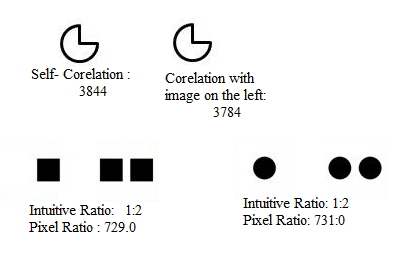
\includegraphics[scale = 0.5]{Images/Fig12}
    \caption{Empirical test to determine the `assumed' threshold values}
  \label{fig12}
\end{figure}

\subsubsection*{A note on the cross corelation measure}
In their paper \cite{paper}, Kunda, McGreggor and Goel had outlined a formula for calculating the similarity score between two frames. The cross-corelation value of the RGB matrices of two frames act as the similarity score in my project, while the self-corelation value of an RGB matrix acts as a baseline for comparison. Using this approach, processing can remain at the lowest level of pixels, instead of having to create abstractions like lines, curves etc., in order to obtain the score.

\subsection*{Implicit Priority}
In case of either 2x2 or 3x3 problems, the order in which the metrics are checked, will impose an implicit prioritization of one metric over the other. For instance, as indicated earlier, the `target' transform for problem 1, is identified as `REFLECTION' instead of `ROTATE90', because the REFLECTION transformation is checked first (ahead of ROTATE90). Similarly for problem 2, the program deduces that the relation is to multiply the existing shape (as opposed to adding a square), because the ratio metric is checked before the difference metric.

\subsection*{Experimental Analysis}
The visual analogy solver was tested against a fairly tough 3x3 problems. The first problem is shown in Figure \ref{exp1}. By splitting up this problem into the individual frames, the analyzer was able to produce the correct answer as 7 (which is right). 
\begin{figure}[h!]
  \centering
    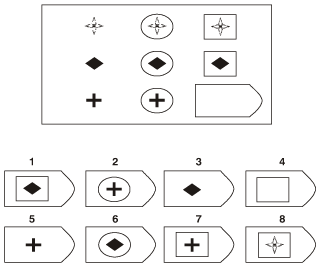
\includegraphics[scale = 0.45]{Images/Exp1}
    \caption{Experimental Problem}
  \label{exp1}
\end{figure}

All 3 metrics, ratio, difference and pair-wise difference were used. The sequence of elimination was,
\begin{enumerate}
	\item Choice 4,5,6,8 were eliminated by the ratio stage.
	\item Choice 1,2 were eliminated by the difference metric.
	\item Between choices 3 and 7, the pairwise difference proved that choice 7's $ChoiceSum$ was closer to the $ReferenceSum$ than that of choice 3.	
\end{enumerate}

\subsection*{Ablation Experiment}
The toughest experimental problem presented to the program is illustrated in Figure \ref{exp2}. The obvious difficulty with this problem is to be able to extract each of the individual frames without loss of information near the boundaries. Also once extracted, it was found that the program gave a completely wrong answer (E as opposed to B). On further inspection, it was observed that there was significantly high levels of noise in each of the answer choice frames. After spending some significant time removing this noise, the program was run again; this time giving the right answer. This clearly indicates that the entire success or failure of the algorithm depends on the quality of the input image.

\begin{figure}[h!]
  \centering
    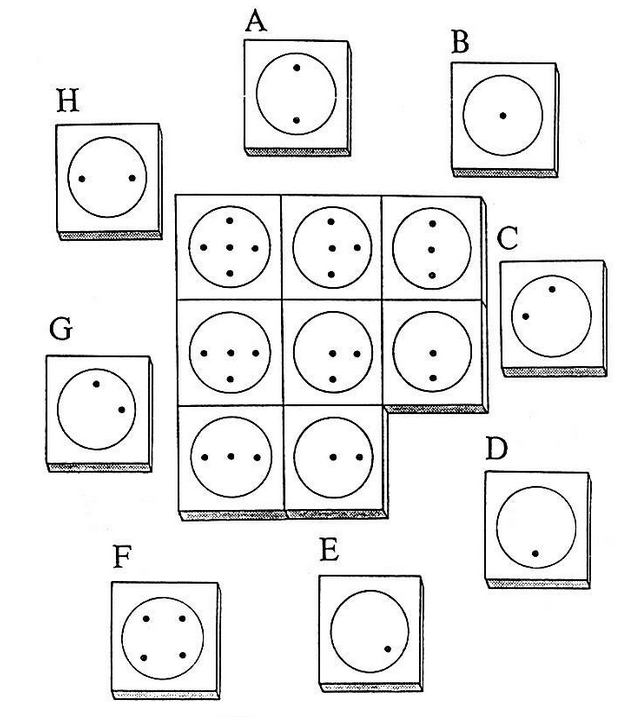
\includegraphics[scale = 0.25]{Images/Exp2}
    \caption{Ablation Experiment}
  \label{exp2}
\end{figure}

\subsection*{Pros and Cons of the algorithm}
	\subsubsection*{Positives}
	\begin{itemize}
		\item Since the algorithm works at the lowest level of abstraction possible - at the pixel level, absolutely no human knowledge or inference is imparted to the system. All inferences made by the system are purely on the merit of the problem.
		\item As the algorithm uses a purely visual representation, the programmer need not spend time in devising a consistent and complete grammar for a propositional representation.
		\item This algorithm can be used with a large degree of generality to solve problems of dimensions 2x2 and 3x3 of varying difficulty levels.
		\item Using corelation measure instead of a simple pixel-by-pixel match significantly speeds up the image comparison process and thereby the overall program execution time is reduced.
	\end{itemize}
	\subsubsection*{Critique of the algorithm}
	\begin{itemize}
		\item The algorithm is highly dependent on the quality of the input images- (a) noise free, (b) relative orientation preserved and (c) all images being of a given dimension. This very restrictive requirement demands from the programmer an insane amount of time to manually process the images before the program even begins to run.
		\item The program still will not be able to uncover subtle relationships that exist among frames (this problem existed with propositional representations too). For example, from Figure \ref{con1}, to a human it is obvious that the relation is that the number of lines of the polygon increases by 1 from left to right and hence the right answer would be having 1 more line than the shape in frame2-1.
Obviously the answer is 3, the hexagon but the program does not print out that answer, irrespective of how noise free the input image is.
\begin{figure}[h!]
  \centering
    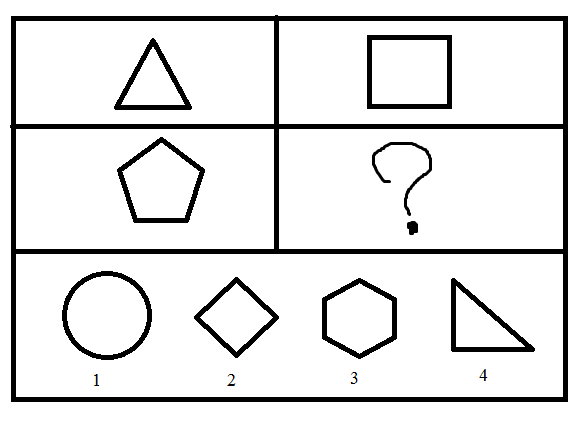
\includegraphics[scale = 0.3]{Images/con1}
    \caption{A subtle relationship that is not uncovered}
  \label{con1}
\end{figure}
		\item The algorithm cannot solve higher dimension analogy problems, which most humans do with some ease.
	\end{itemize}

\begin{thebibliography}{10}
\bibitem{paper} Kunda, Maithilee, Keith McGreggor, and Ashok Goel. "Taking a look (literally!) at the Raven’s intelligence test: Two visual solution strategies." Proc. 32nd Annual Meeting of the Cognitive Science Society, Portland. 2010.

\bibitem{math} Image Compression in JPEG Standard. Retrieved from \url{http://www.whydomath.org/node/wavlets/imagebasics.html}

\bibitem{web} SciPy and NumPy online documentation. Retrieved from \url{http://docs.scipy.org/doc/}

\bibitem{pil} Python Imaging Library. Retrieved from \url{http://www.pythonware.com/products/pil/}

\end{thebibliography}
\end{document}
